%%%%%%%%%%%%%%%%%%%%%%%%%%%%%%%%%%%%%%%%%%%%%%%%%%%%%%%%%%%%%%%%%%%%%%%%%%%%%%%%
% Template for USENIX papers.
%
% History:
%
% - TEMPLATE for Usenix papers, specifically to meet requirements of
%   USENIX '05. originally a template for producing IEEE-format
%   articles using LaTeX. written by Matthew Ward, CS Department,
%   Worcester Polytechnic Institute. adapted by David Beazley for his
%   excellent SWIG paper in Proceedings, Tcl 96. turned into a
%   smartass generic template by De Clarke, with thanks to both the
%   above pioneers. Use at your own risk. Complaints to /dev/null.
%   Make it two column with no page numbering, default is 10 point.
%
% - Munged by Fred Douglis <douglis@research.att.com> 10/97 to
%   separate the .sty file from the LaTeX source template, so that
%   people can more easily include the .sty file into an existing
%   document. Also changed to more closely follow the style guidelines
%   as represented by the Word sample file.
%
% - Note that since 2010, USENIX does not require endnotes. If you
%   want foot of page notes, don't include the endnotes package in the
%   usepackage command, below.
% - This version uses the latex2e styles, not the very ancient 2.09
%   stuff.
%
% - Updated July 2018: Text block size changed from 6.5" to 7"
%
% - Updated Dec 2018 for ATC'19:
%
%   * Revised text to pass HotCRP's auto-formatting check, with
%     hotcrp.settings.submission_form.body_font_size=10pt, and
%     hotcrp.settings.submission_form.line_height=12pt
%
%   * Switched from \endnote-s to \footnote-s to match Usenix's policy.
%
%   * \section* => \begin{abstract} ... \end{abstract}
%
%   * Make template self-contained in terms of bibtex entires, to allow
%     this file to be compiled. (And changing refs style to 'plain'.)
%
%   * Make template self-contained in terms of figures, to
%     allow this file to be compiled. 
%
%   * Added packages for hyperref, embedding fonts, and improving
%     appearance.
%   
%   * Removed outdated text.
%
%%%%%%%%%%%%%%%%%%%%%%%%%%%%%%%%%%%%%%%%%%%%%%%%%%%%%%%%%%%%%%%%%%%%%%%%%%%%%%%%

\documentclass[letterpaper,twocolumn,10pt]{article}
\usepackage{usenix2019_v3}

\setlength {\marginparwidth }{2cm}
\usepackage{todonotes}
% to be able to draw some self-contained figs
\usepackage{tikz}
\usepackage{amsmath}

\newcommand{\iantodo}[1]{\todo[color=green!40]{#1}}
\newcommand{\task}[1]{\todo[inline,color=orange!40]{#1}}
\newcommand{\taskred}[1]{\todo[inline,color=red!40]{#1}}
\raggedbottom

%-------------------------------------------------------------------------------
\begin{document}
%-------------------------------------------------------------------------------

%don't want date printed
\date{}

% make title bold and 14 pt font (Latex default is non-bold, 16 pt)
\title{\Large \bf Everything You Always Wanted to Know About Serverless AI But Were Too Afraid to Ask}
% \title{\Large \bf Agentic Workflows are Serverless Systems, So deploy them that way!}
% \title{\Large \bf Not your parent's serverless AI}
% \title{\Large \bf Who let the AI Agent out on my serverless system?}

%for single author (just remove % characters)
\author{
{\rm Your N.\ Here}\\
Your Institution
\and
{\rm Second Name}\\
Second Institution}

\maketitle

%-------------------------------------------------------------------------------
\begin{abstract}
%-------------------------------------------------------------------------------



% \textbf{Once upon a time.}
Accelerating generative AI adoption has spurred the expansion of datacenters, who amass troves of GPUs, DRAM, and SSDs in an effort to feed emerging resource-hungry AI workloads.
% As the demand for AI continues to grow, so does the burden on datacenters to manage expensive, heterogeneous, and resource-hungry AI workloads. 
The serverless cloud model offers a path to boost the resource efficiency of on-demand applications, enabling hardware sharing between tenants and applications --- however, the suitability of emerging AI workloads on serverless remains insufficiently explored.
% The serverless paradigm, allowing users to pay only for the compute and memory they need, has boosted the resource efficiency of on-demand applications.
% While some AI services, e.g., LLMs, are in high continuous demand, making them a better fit for the “always-on” server model, many other AI workloads, such as small custom models and emerging agentic workloads, may be a good fit for the serverless model. 
% \textbf{Villain}
We survey the state-of-the-art in serverless hosting for text based generative AI and find that:
% (1) Although some serverless deployments of AI workloads currently exist, today's serverless systems are not designed for thei memory hungry, heterogeneous demand.
(1) despite many advancements in serverless LLM hosting, heavy model loading and initialization processes still introduce significant startup latency.
(2) Agentic AI workloads have not yet been characterized under the serverless context.
% \textbf{Hero.}
% We summarize the state-of-the-art on serverless for AI, agentic workloads and other AI workloads fitting to the serverless model.
We propose a deployment scheme for agentic workloads that is tailored for serverless, accompanied with pre-warming policies that minimize idle resource footprint and startup latencies.   
% We present our vision for the future research directions in this space.
This paper outlines our vision for promising research directions in serverless agents. 


% \textbf{Happily ever after}
% We illuminate gaps in serverless deployments for agentic AI, proposing methodologies that increase deployment density and improve SLO attainment.


\end{abstract}


%-------------------------------------------------------------------------------
\section{Introduction}
%-------------------------------------------------------------------------------

% Sasha notes: do better job of tying topic sentences to theme of paper


% \textbf{
% The growth of AI workloads is massive, pushing the development of many datacenters to meet the demand for compute resources.
% }
\textbf{
The growth of generative AI workloads has triggered a colossal shift in computing demand.
}
% the shift is a high demand for accelerators and memory
Generative AI is incredibly resource intensive --- requiring large accelerators, loads of memory, and vast storage capacity.
Additionally, the adoption of AI workflows in industry is accelerating, particularly through the use of text-based agentic applications~\cite{flexera2026cloud, cloudera2025agents, vizard2025agentic}.
To meet the large resource requirements of AI demand, cloud providers are scaling up by building new datacenters and stockpiling hardware~\cite{gvr2023datacenter}.
This shock has manifested in global supply shortages for GPUs, DRAM, and SSDs~\cite{cnbc2026micron, jeronimo2025memory}.
It is clear that to meet the growing demand of AI, we need serving strategies that can more efficiently manage the hardware underlying emerging AI workloads. 

\textbf{
Most AI workloads are executed in the cloud~\cite{kulkarni2021gpu, gartner2022iaas, virtualization2020workloads}, where deployments can fall into one of two categories: always-on or serverless. 
}
In the always-on model, software runs continuously regardless of request traffic. 
In contrast, serverless deployments run only when needed, invoked in response to incoming requests~\cite{kounev2023serverless}.
The serverless model allows hardware to be shared across workloads and tenants, reducing the waste of precious compute resources.
Additionally, serverless users gain the added benefit of flexible billing, paying for the resources consumed.

\textbf{
Still, a gap remains in assessing the suitability of AI workloads to the serverless model. 
}
A precondition of serverless deployments is that client instances should be packageable --- a serverless framework must be able to provision resources and spin up new instances in order to meet incoming request load.
The workloads behind generative AI demand are diverse: spanning LLM inferences, model training and fine tuning, agentic workloads, semantic data stores and more.
We focus on LLM inferences and agentic workloads, as they dominate current AI deployments~\cite{flexera2026cloud, cloudera2025agents, vizard2025agentic} and also show potential for the serverless model.


\textbf{
Recent work has proven the viability of serverless LLM inferencing, primarily for small to medium sized custom models~\cite{serverlessllm, deepserve, serverlesslora, slinfer, hydraserve, wages, prewarm-not-enough, pipeboost}.
}
On-demand loading of large LLMs can cause significant cold-start delays, where requests must wait on standby for model initialization before they are serviced.
Additionally, the large request footprint of each individual model can cause GPU contention during periods of high load.
% Not all LLMs are suitable for serverless, large closed weight models such as ChatGPT~\cite{chatgpt}, Gemini~\cite{gemini}, and Claude~\cite{claude} see continuous demand, aligning closely with always-on deployments.
Recent work alleviates some of these costs~\cite{serverlessllm, deepserve, serverlesslora, slinfer, hydraserve, wages, prewarm-not-enough, pipeboost}, however we find that model cold starts remain a challenge.
Small to mid-sized models show promise in both mitigating startup times, resource footprints, and are increasingly popular.
We view recent trends in using small fine tuned models for agent task execution~\cite{belcak2025smalllanguagemodelsfuture} driving the deployment of many application-specific serverless LLM deployments.  

\textbf{
As a driving force behind current AI demand, extending agents into serverless deployments offers enormous potential for reducing the resource footprint of AI.
% The applicability of agentic workloads to the serverless framework remains largely unexplored, despite being a driving force behind current AI demand~\cite{cloudera2025agents, vizard2025agentic}.
}
Agents are distinct from traditional serverless workloads in a number of ways; they rely on heterogeneous compute while exhibiting non-deterministic and long running behavior.
A number of optimizations have been proposed to improve agent serving at scale~\cite{raj2026understandinganalyzingoptimizingagentic, wei2026agentxpuefficientschedulingagentic, wadlom2026efficientllmservingagentic, pagonas2025cortexworkflowawareresourcepooling}, however extending agents to the serverless model remains largely unexplored. 
% Agents depend on many other services for context.
% How can agentic workloads be characterized, resource footprint and execution times.
% What is the best deployment configuration?

In this paper we contribute the following:
\begin{itemize}
    \item We summarize the state of the art in serverless LLM hosting, covering an array of cold start mitigation techniques and serving density optimizations.
    \item We present practical serverless deployment scenarios for agents and illustrate hidden challenges in serving agentic workloads.
    \item We perform a workload characterization of representative agentic workloads, guiding the selection of serverless policies.
\end{itemize}

% \task{Still need to connect why this paper puts dual focus on LLMs \& agents.}

%-------------------------------------------------------------------------------
\section{State of the Art}
%-------------------------------------------------------------------------------

% writing group
% pros:
% prefill + decode came across clear
% inference explanation comes across
% statistic was strong! maybe i need more


% cons:
% table to draw parallels from serverless to serverless LLMs, 
% add empirical data to agent section
% agent serving sentence is not super clear 



% \subsection{Workflows}
% \task{It's probably useful to see whether the different usages actually result into different usage patterns}
% We may have different workload patterns. Need to verify this. Typically, there are foreground and background tasks, but with agents, there seems to be a third class that has some characteristics of both. 
% \begin{description}
%     \item[User-Initiated] This is basically a user asking the LLM for things. a bit like search. This may trigger some web searches or similar. This might also be like a short-ish agent. Should produce results in near-real-time. 
%     \item[Agent-Initiated] This might be more of a "fast" user? possibly even with some more parallelism. Here, results should be returned within a reasonable amount of time.  Here we could also view this as START-USE-STOP.  Also, we seem to know the workflow, that we can use to pre-warm. 
%     \item[Batch] we can decide when to schedule this. Latency doesn't quite matter.
%       -> could we use an idle-pre-warmed LLM instance to run the batch job (maybe it can be pre-empted)

% \end{description}

\subsection{Traditional Serverless}


\textbf{
Through revisiting the decade of innovation in the traditional serverless domain, we can envision solutions to parallel problems in serverless AI hosting. 
}
% \textbf{
Serverless computing has become an immensely well established business model offering flexible pay-as-you-go compute~\cite{kounev2023serverless, googlecloudfunctions, azurefunctions, openwhisk, firecracker}.
% }
Custom functions are uploaded by clients and cloud providers automatically handle resource provisioning and instance scaling as requests arrive.
The sharing of underlying compute resources between function instances and tenants allows for greater serving efficiency, but also exposes challenges for function isolation and request response times.
Requests must be serviced within a specified time frame determined by the provider's Service Level Objectives (SLO), but ideally these requests are handled with a minimum number of machines to most efficiently use the available compute resources.
Hence, serverless systems crucially rely on instance placement and autoscaling policies to schedule function instances as requests stream in.

\textbf{
A circular dilemma arises in the serverless paradigm: the long-tail clients that benefit the most from flexible billing are ironically the most challenging to effectively serve.
}
Before a request can be serviced, both the serverless runtime and client function must be loaded and initialized.
However, function instances that are infrequently invoked will not stay loaded, leading to cold start delays as requests wait for instances to spin up.

\textbf{
The cold-start problem has inspired a large number of widely accepted policies to handle function loading and scaling.
}
Since requests feature bursty arrival patterns, keeping instances warm in DRAM for a keep-alive timeout can obviate subsequent cold starts~\cite{lambda, faascache}.
Opportunistic pre-warming can be used to predictively load instance data before requests arrive~\cite{recycle-containers, prewarm-not-enough}.
Additionally, more functions can be kept warm in DRAM through memory deduplication between instances~\cite{lambda, medes, qiu2023userguidedpagemergingmemory}.

\textbf{
Alternatively, cold start latency can be attacked head-on by optimizing function loading.
}
Function virtualization between tenants is traditionally provided by containers, but lightweight virtualized language runtimes can be used instead to circumvent heavy container initialization costs~\cite{virtines, firecracker, catalyzer}.

\subsection{Anatomy of an LLM Inference}

\textbf{
LLM inferences are heavyweight, complicated operations that play a central role in generative AI serving. 
}
Understanding the internal structure of an inference is foundational to many systems optimizations for serving LLMs.
We divide an inference into 3 stages: initialization (which is performed once at model load time), prefill, and decode --- the latter two of which occur on every inference.

\paragraph{Initialization}
Before inference can start, the inference engine must load model weights into VRAM.
This process is costly, as model weight files are large, reaching hundreds of gigabytes at the top end.
In addition, the inference engine initializes two more optimizations.
The first is the capturing of a CUDA graph, which defines the command sequence of kernels launched by the CPU during inference.
Capturing the CUDA graph allows kernels to be launched on the GPU, eliminating the communication bottleneck between the CPU and GPU~\cite{vllm, medusa}.
The second optimization is the preallocation of VRAM for the KV cache.
% engines: vLLM TensorRT LLM llama.cpp
% Modern inference engines like vLLM offer "PagedAttention"~\cite{vLLM}, enabling OS-like virtual memory for LLM inferences on GPUs.
% Not all model weights need to be in VRAM, it is common for only a subset of weights to be active in mixture of expert (MoE) models.

\textbf{Prefill}
The prefill stage ingests the prompt, builds the KV cache, and predicts the first token of the response.
This stage is compute bound, as the entire prompt is processed in parallel.
The KV cache is an essential datastructure for LLM inferences, storing intermediate state that would otherwise require duplicate computation during each forward pass of the decode stage.

\textbf{Decode}
The decode stage is the autoregressive process by which each token is generated.
Each step takes the last token, queries the KV cache, predicts the next token, and updates the KV cache until an termination token is generated.
This stage is memory bandwidth bound, and determines the throughput of the inference.

\task{what do i need to remember?}

\task{inference figure breakdown of stages}

\subsection{Serverless LLMs}

\textbf{
As the community around open weight models has matured, the demand for custom cloud inference solutions has emerged.
}
In 2025 alone, the number of models hosted on Hugging Face doubled \cite{rios2025huggingface}.
This trend reveals a broad interest in open weight LLMs, however hosting a large catalog of LLMs remains challenging.
% With many models competing for limited GPU space, serverless inferencing solutions face large cold start penalties and high resource footprints. 
% move big LLM ideas to intro
% \textbf{
% The services that provide inferences for closed weight models like ChatGPT, Gemini, and Claude are conceptually parallel to serverless LLMs --- users pay at the granularity of tokens, only for the inferences requested.
% }
% These services still require robust autoscalers to respond to variable request load, but with a small number of models the cold-start problem is much simpler to address.
% For a small model catalog, keeping models warm in GPU memory is feasible, circumventing model loading costs.
A serverless system that hosts inferences for custom LLMs does not have the luxury of fitting warm model instances in GPU memory.
At production scale, there can be thousands of custom models to serve~\cite{deepserve}, with many experiencing sparse request patterns~\cite{zheng2024lmsyschat1mlargescalerealworldllm, xiang2025servegenworkloadcharacterizationgeneration, wang2025burstgptrealworldworkloaddataset}.
The challenge of building serverless LLM infrastructure that mitigates cold-starts and efficiency utilizes compute has seen a lot of recent attention.
We provide an overview of recent work in serverless LLMs:

\newcommand{\ServerlessLLM}{\textsc{ServerlessLLM}}
\newcommand{\HydraServe}{\textsc{HydraServe}}
\newcommand{\DEEPSERVE}{\textsc{DeepServe}}
\newcommand{\ServerlessLoRA}{\textsc{ServerlessLoRA}}
\newcommand{\PipeBoost}{\textsc{PipeBoost}}
\newcommand{\Medusa}{\textsc{Medusa}}
\newcommand{\InstaInfer}{\textsc{InstaInfer}}
\newcommand{\SLINFER}{\textsc{Slinfer}}
\newcommand{\WAGES}{\textsc{Wages}}
\newcommand{\Torpor}{\textsc{Torpor}}
\newcommand{\lambdascale}{\textsc{$\lambda$Scale}}

\paragraph{Model Loading.}
Loading model parameters into GPU memory is the single largest contributor to cold start latency for large LLMs.
The cost of shipping model weights into GPU memory prior can easily dwarf the cost of a single inference.
Model loading times can be partially mitigated through effective management of a GPU node's deep storage hierarchy.
Prior to inference, a model checkpoint may live in VRAM, DRAM, on disk, or in remote storage; each storage tier varies by an order of magnitude in model loading speed~\cite{deepserve}.

\ServerlessLLM~\cite{serverlessllm} routes requests to nodes where model checkpoints are local, avoiding costly model loading from remote storage.
% In cases where a request is routed to a busy node, live migration of inferences over high bandwidth GPU-GPU links can be used to create space for incoming requests.
When loading from remote storage is necessary, \HydraServe~\cite{hydraserve} provides an optimization through aggregating multiple peers' network bandwidth.
Model checkpoints are distributed among peer nodes, and new instances are placed on nodes that minimize network contention.
% Data movement during model loading can saturate network bandwidth, so the authors design a network contention aware policy for worker placement that minimizes SLO violations stemming from network interference.

High bandwidth GPU-GPU links are a powerful mechanism for moving model weights that are already present within one accelerator's memory.
These links can be used for rapid horizontal scaling in response to request bursts \cite{yu2026lambdascaleenablingfastscaling, deepserve}, achieving over 10$\times$ speedup for model loading at 72 billion parameters.
% \lambdascale \DEEPSERVE~\cite{deepserve}, Huawei's production serverless LLM solution, implements multiple model loading optimizations to minimize cold start times.
% In addition to proactively loading models into DRAM, \DEEPSERVE~uses high bandwidth NPU-NPU links to scale out running instances in response to load bursts.
% The NPU-fork path proves to be an order of magnitude faster than loading from DRAM.
Alternatively, high bandwidth links can be used to migrate inferences to create space for new instances to be loaded from local DRAM~\cite{serverlessllm}.

\task{The current state of model cold starts: unless a model is already loaded in VRAM, or on a GPU's peer node (high-bandwidth network topology dependent), cold start times are still highly punitive.}

\task{
table of cold start times across model sizes and where it is loaded from
}

\paragraph{Model Initialization.}
LLM inference engine initialization lies on the cold-start path for newly loaded models. 
\Medusa~\cite{medusa} targets this initialization overhead with materialization, delegating a portion of the initialization to offline preprocessing.
\Medusa~introduces optimizations to remove dynamic memory management during KV cache creation, and further parallelizes this stage alongside model loading.
Similarly, CUDA graphs are consistent in structure between consecutive model loads, but still hold runtime dependencies on dynamically determined data pointer values.
\Medusa~addresses non-determinism by inserting a shim layer to abstract runtime dependent kernel parameters.

\task{medusa claims higher initialization costs than every other paper, i see gpt-oss-20b cuda capture on our A100 at \~20s, consistent with medusa. do all other papers forgo cuda graph capture?}

\paragraph{Pre-warming.}
Serverless orchestrators can proactively load instance data into DRAM in anticipation of future requests, drastically reducing container loading overhead.
This practice, called pre-warming, is an established, industry recognized technique in traditional serverless systems to mitigate cold starts.
Naturally, serverless LLMs have also adopted pre-warming.

\DEEPSERVE \cite{deepserve} implements pre-warming natively by predictively loading up to 1.5TB worth of models to DRAM.
Unfortunately for LLM inferences, even if the model is present in DRAM, loading to GPU memory can still take significant time.
Many prior works assume DRAM pre-warming as an implicit starting point for cold start optimizations~\cite{serverlesslora, pipeboost, medusa, slinfer}.

\InstaInfer \cite{prewarm-not-enough} surpasses pre-warming and proposes pre-loading model data directly to the GPU.
\InstaInfer~does not evaluate against LLMs, but the technique shows promise for other ML inference workloads.

\paragraph{Serving Density.}
The heterogeneous nature of LLM inference creates a significant imbalance in resource utilization.
LLM inferences compete for GPU time, leaving CPU compute underutilized.
Harvesting this spare compute is as an opportunity to increase serving capacity in serverless systems.
\SLINFER~\cite{slinfer} demonstrates that CPUs equipped with matrix accelerators (Intel AMX) can serve small to mid sized LLMs without violating SLOs.

CPU compute is not the only underutilized resource, the memory bandwidth heavy nature of LLM inference leaves plenty of GPU compute headroom \cite{llama3}.
\WAGES~explores GPU sharing through NVIDIA Multi-Process Service (MPS), partitioning GPUs into multiple instances for simultaneous inference of multiple models~\cite{wages}.
Additionally, GPUs expose fine grained frequency controls, which \WAGES~leverages to minimize energy consumption during LLM execution.

% conceptual parallel to memory deduplication in the classic sense
% provide context here, this effectively reduces the number of base models one must deploy
% LoRA~\cite{lora}, a popular fine tuning technique, explicitly freezes the weights of the base model during training and updates only a small number of new low rank matrices.
Another angle for optimization lies in the duplication of parameters between models.
In particular, fine tuned models derived from the same base model share over 99\% of parameters \cite{serverlesslora}.
\ServerlessLoRA~\cite{serverlesslora} leverages this to isolate the loading stages of base models from their fine tuned parameters.
By keeping base models loaded in GPU memory, additional inferences can be served by just loading the fine tuned layers, reducing cold start delays and increasing deployment density.
\PipeBoost~\cite{pipeboost} takes this idea further, and allows for inference to start on the GPU in parallel with the loading of the fine tuned layers.

\task{\Torpor{} project}

% \subsection{Agentic Workloads}

% LLM inferences are only one component of broader AI applications.
% Raw inferences are extended through agentic environments that allow tool usage through aaaaaaaaaaa 


\subsection{Agent Serving}

\newcommand{\helium}{\textsc{Helium}}
\newcommand{\cortex}{\textsc{Cortex}}
\newcommand{\parrot}{\textsc{Parrot}}
\newcommand{\autellix}{\textsc{Autellix}}
\newcommand{\halo}{\textsc{Halo}}

\textbf{
Agentic workloads can vary greatly in architecture and capabilities.
}
For our purposes, we define agents to be any logic that encapsulates and extends an LLM inference.
This can include tool calling and actions but does not strictly require it.
Some agents follow a predefined static path, while others have dynamic and recursive workflows dependent on the input query.
Additionally the resources used by agents can span a large domain of complexity and resource intensity.
An agent may perform simple web searches over the network, invoke approximate nearest neighbor queries into a vector database, or spin up a local container for code execution.

% \task{table of popular tool calls and the corresponding resource requirements. A non-exhaustive list: 
% LLM inferences, embedding inferences, Vector DBs, Knowledge graphs, relational DBs, web APIs, code execution environments (python E2B or Open Interpreter), calculators, other agents}

\textbf{
Existing LLM serving systems optimize for single-shot inference, overlooking the broader application context available in agentic workflows.
}
Many works have explored how application context can be effectively utilized from the inference serving perspective, where a model is already initialized and fielding many inference requests.

\textbf{
Decomposing agentic workloads into their component stages reveals scheduling opportunities to more effectively use underlying hardware.
}
% At a high level, agentic workloads are heterogeneous and dynamic, however the individual resource footprint of each workflow stage is much more predictable.
The stages of agentic workflows can be effectively captured as a directed acyclic graph (DAG), where nodes perform inferences, execute tools calls, or wait on user input.
Several works leverage an agent's DAG to schedule inferences, improving overall response times through batching highly-parallel inductive phases and boosting the priority of final deductive inferences~\cite{lin2024parrotefficientservingllmbased, luo2025autellixefficientservingengine, wadlom2026efficientllmservingagentic}.

\textbf{
Agentic workloads feature interdependent LLM calls, where significant portions of prompts are reused, allowing for intermediate inference results to be shared across inferences~\cite{wadlom2026efficientllmservingagentic, pagonas2025cortexworkflowawareresourcepooling, lin2024parrotefficientservingllmbased, luo2025autellixefficientservingengine, peng2026hexgenflowoptimizingllminference}.
}
Context is reused across both intra-request inferences, as task specific context overlaps between subsequent workflow stages, and also across request boundaries, as agents reapply system prompts to handle new user tasks.
% \parrot{} finds that between different users, production prompts share over 94\% of tokens \cite{parrot}.
\cortex{} advocates for stage isolation, routing all inferences of each stage to dedicated inference engines, implicitly improving KV cache hit rate~\cite{pagonas2025cortexworkflowawareresourcepooling}.
Alternatively, KV cache reuse can be treated as a first class citizen; \helium{} analyzes workflow stages for prompt similarity and collocates similar inferences on the same engine~\cite{wadlom2026efficientllmservingagentic}. Additionally, \helium{} implements a proactive caching strategy that precomputes KV cache data for the static portion of agent prompts, these results are cached globally and proactively loaded into GPU memory as the inference engine fields similar requests.

% \textbf{
% Despite the GPU intensive nature of inference operations, the role of the CPU as a central orchestrator can actually become a source of bottlenecks in agent execution~\cite{raj2026understandinganalyzingoptimizingagentic}.
% }
% Tool usage can call into other highly expensive operations: code execution.

% \textbf{
% analogies to DBMS community
% }
% DAG execution
% Throughput vs latency = OLTP vs OLAP


\section{Characterizing Agentic Resource Footprint}
\textbf{
We present a case study over three representative agentic workloads.
}
These have been chosen to vary in workflow complexity and in tool use.

\begin{description}
    \item[Haystack RAG]
    User Query -> Query Embedding -> ANN Search -> Document Retrieval -> LLM inference.
    simple, deterministic execution, relies on embedding generation, vector db ANN lookup, and LLM inference.
    Three resources that need to be dynamically loaded in a serverless context.
    \item[Mini SWE agent]
    User Query -> Build context from code/past executions -> LLM inference -> tool calls (execute bash script) -> repeat until LLM determines stopping.
    linear iteration loop, relies on a sandboxed code execution environment and an LLM.
    Variable number of iterations.
    \item[GPT-Researcher]
    User Query -> Planning LLM inference -> Parallel Execution agents (make web queries, and summarize results) -> build big prompt for final LLM summarization step.
    Branching agentic calls with orchestrator LLM.
\end{description}

\begin{figure}[ht!]
    \centering
    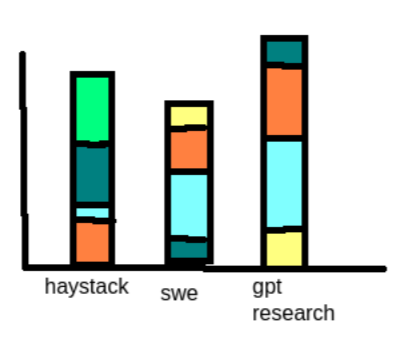
\includegraphics[width=0.7\columnwidth]{./temp-execution-times.png}
    \caption{Execution times of agentic workloads broken down by inferences and tool use.}
    \label{fig:bench-execution-times}
\end{figure}

\begin{figure}[ht!]
    \centering
    \textbf{CPU Utilization: }\\
    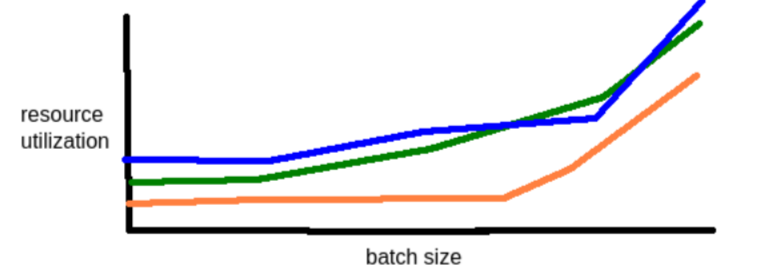
\includegraphics[width=0.8\columnwidth]{./temp-utilization.png}\\
    \textbf{DRAM Utilization: }\\
    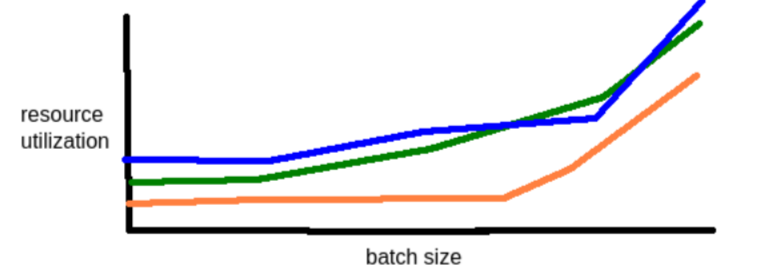
\includegraphics[width=0.8\columnwidth]{./temp-utilization.png}\\
    \textbf{GPU Utilization: }\\
    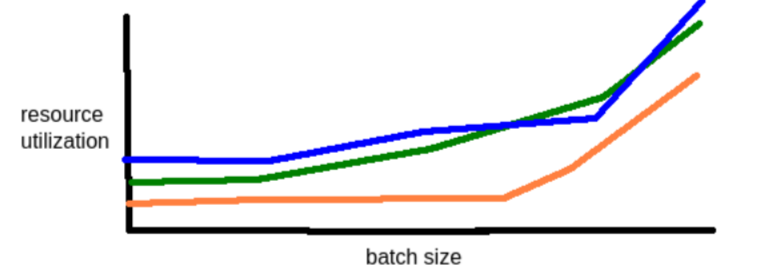
\includegraphics[width=0.8\columnwidth]{./temp-utilization.png}\\
    \textbf{VRAM Utilization: }\\
    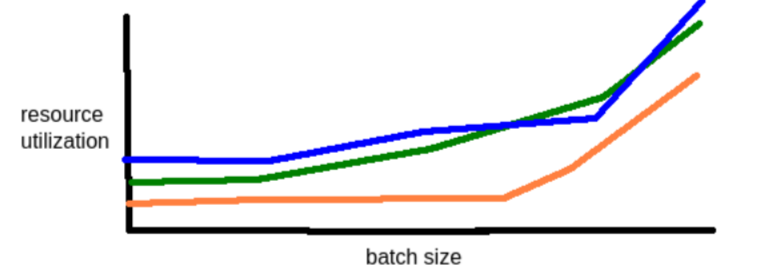
\includegraphics[width=0.8\columnwidth]{./temp-utilization.png}
    \caption{Resource usage of agentic workloads as batched requests increase.}
    \label{fig:bench-execution-times}
\end{figure}

\task{figure of all workloads, latency of each step, followed by memory and compute resources for each step}

\task{
Include a figure of agent dag with tool use, where those tools run.
}

\subsection{Traces}

\paragraph{Session Length} Available for LLM chats but not for 

\paragraph{Agent topologies} Somewhat available through public langsmith records, no central repos though

\paragraph{Inference Input/Output Lengths} Proxy for execution times, informs

\paragraph{Call for Agent Traces} There is a gap in publicly available trace info. We need more traces that capture resource usage, timing, and agent workflow topology in order for the systems community to design solutions.

% \subsection{Model Choice}

% \textbf{
% Picking the LLM to drive an agent is potentially the most impactful decision for both agent accuracy and execution performance.
% }
% The right model varies by task complexity and performance requirements.
% Large reasoning models offer strong task performance, but can be expensive for inference due to long reasoning traces.
% Recent works have shown viability in using small LLMs to drive agentic workflows.
% % https://arxiv.org/pdf/2506.02153
% Agents may even invoke multiple models in adversarial roles to refine answers.

% \textbf{
% The choice of model is also incredibly impactful in a serverless context, determining different potential optimizations.
% }
% Large models are particularly difficult to load in the cold-start case.
% Small models are faster to load, but also can potentially be executed on the CPU.
% Fine tuned models can be memory deduplicated from one another, offering more efficient pre-warming.
% Mixture of expert models only require a subset of active parameters to be loaded on the GPU, cutting down loading times and increasing VRAM headroom for sharing.


\section{A Vision For Serverless Agents}
\task{pull insights from serverless LLM traces as motivation in this section}

\textbf{
Agents are the dominant workload driving AI demand; improving the resource efficiency of agents under the serverless model has potential for mitigating the broader resource footprint of AI.
}
Most prior work addresses agent serving from the model inference perspective, however the role of the CPU as a central orchestrator can actually become a source of bottlenecks in agent execution~\cite{raj2026understandinganalyzingoptimizingagentic}.
We propose using the structured nature of agentic workloads to improve resource efficiency and cold start latency through selectively pre-warming workflow stages.

% agents are long running with variable resource usage, a monolithic deployment may inefficiently utilize provisioned resources

\textbf{
}

\subsection{Monolithic vs Modular Deployments}

\textbf{
An agent can be deployed in a serverless system just as any other function, through isolating CPU orchestration and tooling logic.
}
Serverless agents may make external API calls for subtasks that require heterogeneous compute or persistence: LLM inference through paid token APIs~\cite{chatgpt, gemini, claude}, custom models hosted on a serverless LLM platform~\cite{deepserve, amazonbedrock, ocigenai, anyscale}, vector databases, document stores, or any number of external resources.
We refer to this methodology, where all workflow stages are bundled into one package, as the monolithic deployment.
All serverless scheduling decisions for instance loading, horizontal scaling, and keep-alive must operate on the entire agent's container.

\textbf{
Alternatively, serverless agent deployments can be deconstructed into each workflow's component stages for greater resource efficiency.
}
The representation of agentic workloads as DAGs is well supported in agent serving literature~\cite{lin2024parrotefficientservingllmbased, luo2025autellixefficientservingengine, wadlom2026efficientllmservingagentic}, where each node represents an LLM inference, tool execution, or user interaction.
Under this modular deployment strategy, each workflow stage has the flexibility to be loaded, scaled, or unloaded independently.


\textbf{
Consider a keep-alive policy that selectively keeps the first agent stage warm in DRAM: when a request is fielded, the first stage can execute immediately while latter workflow stages load in parallel.
}
The resource footprint of a partially warm instance is dramatically reduced while maintaining the performance of the monolithic deployment.

\textbf{
A similar argument holds for container cold starts. When a request is received for a cold instance, only the first stage must be initialized before function execution begins.
}
Subsequent model stages can load in parallel, mitigating the cold start latency compared the coarse loading of monolithic agent deployments.

\subsection{Small Language Models}

\textbf{
Despite the industry dominance of large generalist models, small custom models show strong performance on agentic workloads at a fraction of the size~\cite{belcak2025smalllanguagemodelsfuture}.
}
The trend towards small language model (SLM) usage in agents is motivated by faster inference speeds and smaller resource footprints at competitive application performance~\cite{belcak2025smalllanguagemodelsfuture}.
Fine tuned SLMs are an efficient alternative for agentic subtasks that are narrowly scoped and do not require the generality of LLMs.
Support for SLMs is crucial to sustainably meet today's AI demand.
We argue that serverless infrastructure for agents should be designed with the deployment of custom SLMs in mind.

\textbf{
SLMs are a natural fit for serverless deployment; they are lightweight and custom to individual tenants.
}
A number of additional benefits are available for agent SLMs:
they are small enough for practical CPU inference~\cite{slinfer}, many models can be pre-warmed into DRAM simultaneously, and shared base model weights can be deduplicated for substantial memory savings.

\textbf{
Cold starts for serverless SLM deployments can be effectively mitigated through codesign with serverless agents.
}
The lifetime of a serverless SLM can be treated as another modular stage in the agent workflow, removing the guesswork from SLM scaling. 
When a cold agent instance is invoked, the SLM can be loaded onto a GPU immediately instead of waiting for the first inference API call.
Additionally, SLM instances can be confidently unloaded when upstream agent instances are unloaded.

\subsection{Serverless Closures}

\paragraph{Workflow Loading} How much state is captured in an interactive agent run?

\paragraph{KV Cache Offloading} \helium{} style pre-processing and KV cache storage.

\subsection{Scheduling}

\paragraph{Cold Starts}
\paragraph{Autoscaling}
\paragraph{Function Migration}


% \paragraph{Industry Traces?}
% % Notes:
% % servegen argues that per tenant request patterns stay relatively stable
% % this motivates keepalive policies by tenant
% % keepalive can block new requests. (keep KV cache around, keep model loaded)
% % many existing works implicitly mention prewarming (models to dram), but few provide a real policy for doing so

% \begin{itemize}
%     \item not sure yet if this should be in related work or elsewhere as supporting analysis
%     \item LMSYS, ServeGen (Alibaba), BurstGPT (Azure)
% \end{itemize}


% \subsection{Autoscaling}

% \textbf{
% The nondeterministic execution of agents makes instance scaling challenging.
% }
% Agents can spin off long running jobs that process large corpuses of data or they can perform a simple task and yield control.
% This variation response times is inherent in the varied task complexity that agents are designed to solve.
% How do you know if you have enough compute allocated to meet incoming request load?

% \textbf{
% The concept of an SLO for serverless agents is not well defined.
% }
% Time to First Token (TTFT) and Tokens per Second (TPS) are well established metrics for LLM performance.
% These metrics work well in simple cases like chat interfaces, but can break down in agentic workloads that produce large non-text artifacts.
% The tolerable performance for an agent may vary wildly depending on the application.

% \textbf{
% Vertical scaling can be achieved through request batching \cite{raj2026understandinganalyzingoptimizingagentic}.
% }
% Batching is an effective mechanism for increasing throughput across many of an agent's tools.
% Inference batching can increase GPU utilization, query batching for databases can reduce individual request overheads.

% \textbf{
% Horizontal scaling is a necessary mechanism in serverless systems when the request load outgrows the resources of a single machine.
% }
% The threshold to scale horizontally is complicated within agentic systems due to the variability of resource footprint between individual requests.
% Agent migration can be a useful tool when scaling out and reconsolidating, especially given the long lifespan of agents.

% \subsection{Instance Placement}

% \textbf{
% Agents are incredibly heterogeneous in nature, making function placement more challenging than 2D bin packing of compute x memory.
% }
% Where should agentic logic be placed? Should it be colocated with LLM execution?

% \textbf{
% Agentic logic can be colocated with LLM inferences where CPUs remain underutilized.
% }

% \textbf{
% The prevalence of small agentic LLMs opens the door for CPU inference.
% }
% One-off agent instances are better suited to CPU to prevent model loading times, well trafficked agents benefit from GPU inference where throughput can be sustained.

% \textbf{
% Agents depend on other serverless instances for some workflow stages: models, storage, and other agents.
% }
% In the traditional serverless setting, this feature is known as function chains.
% Prior literature shows that colocating function chains can decrease network contention and improve latency. 


% \subsection{Tenant Isolation}

% \subsection{Agent-Inference Codesign}

% \textbf{
% Through co-designing serverless agents and serverless LLM inferencing platforms, opportunities are exposed to mitigate model cold-starts and improve resource utilization.
% }

% \textbf{
% Models can be prewarmed as agent instances are starting up, opening up pipeline parallelism to reduce model cold-starts.
% }
% We find in our sample workloads that many agents perform tasks before invoking an LLM inference, commonly to retrieve data in order to build a model context.
% Even though the end to end performance of agentic workloads is highly variable, individual workflow steps can exhibit more predictable steps.
% Tapping into this determinism can allow a co-designed serverless platform to effectively the lifetime of agent dependencies to the execution of agents themselves.
% Similarly, requests to agents can be used to proactively drive scaling decisions for downstream serverless instances. 

% \textbf{
% KV caches can be stored as persistent function state, reducing prefill time and improving TTFT.
% }
% Agents reuse system prompts over successive requests, allowing for KV caches to be effectively reused as well.
% Particularly the reuse of KV caches may aid the performance of CPU inference, as CPUs struggle with the compute bound prefill stage.



\section{Conclusion}


%-------------------------------------------------------------------------------
% \bibliographystyle{plain}
\bibliographystyle{unsrt}
\bibliography{references}

%%%%%%%%%%%%%%%%%%%%%%%%%%%%%%%%%%%%%%%%%%%%%%%%%%%%%%%%%%%%%%%%%%%%%%%%%%%%%%%%
\end{document}
%%%%%%%%%%%%%%%%%%%%%%%%%%%%%%%%%%%%%%%%%%%%%%%%%%%%%%%%%%%%%%%%%%%%%%%%%%%%%%%%

%%  LocalWords:  endnotes includegraphics fread ptr nobj noindent
%%  LocalWords:  pdflatex acks

